Exercise 2 addresses implementing a parallel algorithm for blurring images.
The original image, which is used in the exercise is presented on \cref{fig:ex2-before}.
The image blurring process can be done in different ways, however for this excise, the \textit{neighbor weighted average} technique is used.
It is done, by taking the pixel representation of an image, as illustrated on \cref{fig:ex2}, and for each pixel, multiply the selected pixel and its surrounding pixels with predefined weighted values:

\begin{align*}
\omega_{avg} &= (\omega_1 \cdot p_1) + (\omega_2 \cdot p_2) + ... + (\omega_N \cdot p_N) 
\end{align*} 

Once these weighted pixel values are calcdaulated, they are added together to define the new blurred pixel value for the center pixel. 
By performing this operation onto every pixel of the original image, the resulted blurred image is seen on \cref{fig:ex2-after}.
The averaging through neighbor weighted average is expressed naturally using a parallel stencil operation as described in \cref{sec-stencil}.
The weighing filter can have various appearances, however the one used in the exercise is shown on \cref{fig:ex2} marked with blue colors.

\begin{figure}[ht]
	\centering
	\begin{subfigure}{.5\textwidth}
		\centering
		\fbox{
			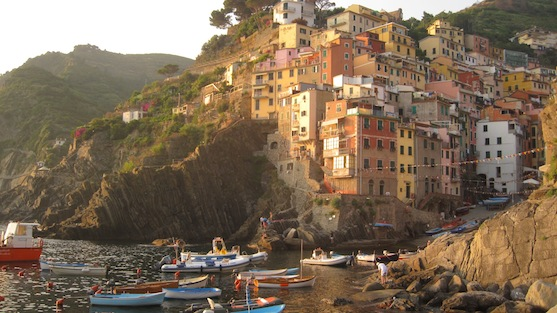
\includegraphics[width=0.8\textwidth]{figs/exercises/ex2/cinque_terre_small.jpg}
		}
		\caption{Before}
		\label{fig:ex2-before}
	\end{subfigure}%
	\begin{subfigure}{.5\textwidth}
		\centering
		\fbox{
			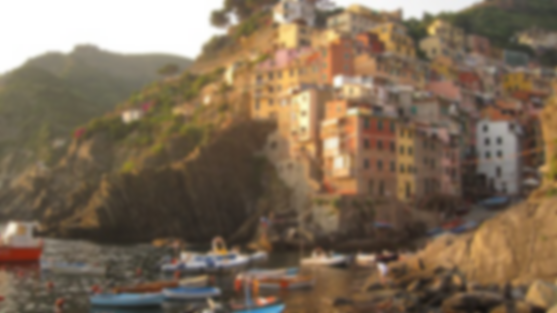
\includegraphics[width=0.8\textwidth]{figs/exercises/ex2/HW2_output.png}
		}
		\caption{After}
		\label{fig:ex2-after}
	\end{subfigure}
	\caption{Picture before and after blur effect is added}
	\label{fig:ex4}
\end{figure}

\begin{figure}[ht]
	\centering
	\fbox{
		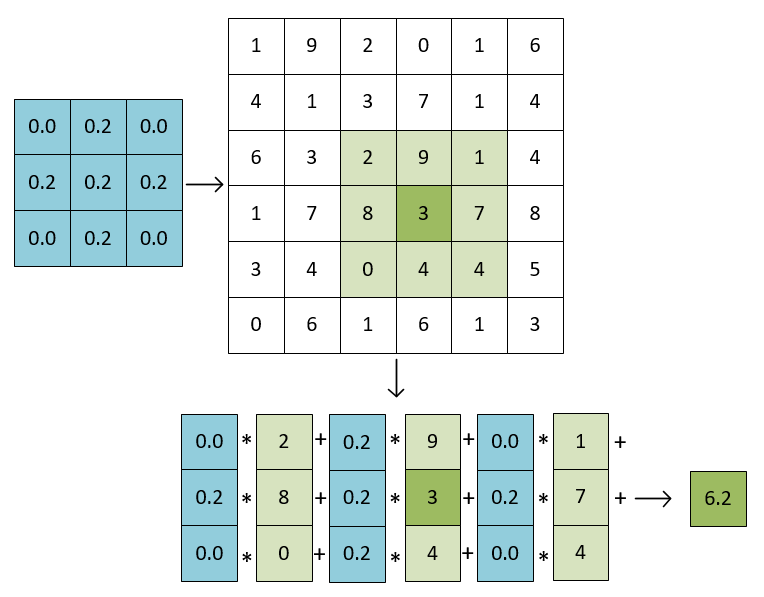
\includegraphics[width=0.8\textwidth]{figs/exercises/ex2/hw2.PNG}
	}
	\caption{Weighing filtering}
	\label{fig:ex2}
\end{figure}

Prior to the blurring itself, the colored image is separated in the three color channels red, green \& blue, in order to store each color contiguously instead of having it interleaved, which is done to simplify the remaining exercise.
\\\\
The exercise is separated into four steps, which are presented below, to see the entire source code of the exercise, see \cite{exercises}.

\begin{enumerate}
	\item[\textbf{Step 1}] First write a kernel to separate a colored image into R, G \& B channels.

	\item[\textbf{Step 2}] Next step is to write the blurring kernel, running through all pixels and perform the blurring filtering described earlier.
	Here care must be taken to clamp neighboring values to be within the bounds of the image, to ensure no reads of neighboring pixel values lying outside of the image is performed. 
	

	\item[\textbf{Step 3}] The third step is to allocate memory for the filter used.
	This should be done using \texttt{cudaMalloc} as described in \cref{sec-pm-memory} and ensuring nothing goes wrong by using \texttt{checkCudaErrors}.

	\item[\textbf{Step 4}] Last step is to compute the optimum grid size based on the image size and the block size.
	Finally, the three blurred channels are combined to create the blurred final image.
\end{enumerate}

